\begin{figure}[H]
\centering
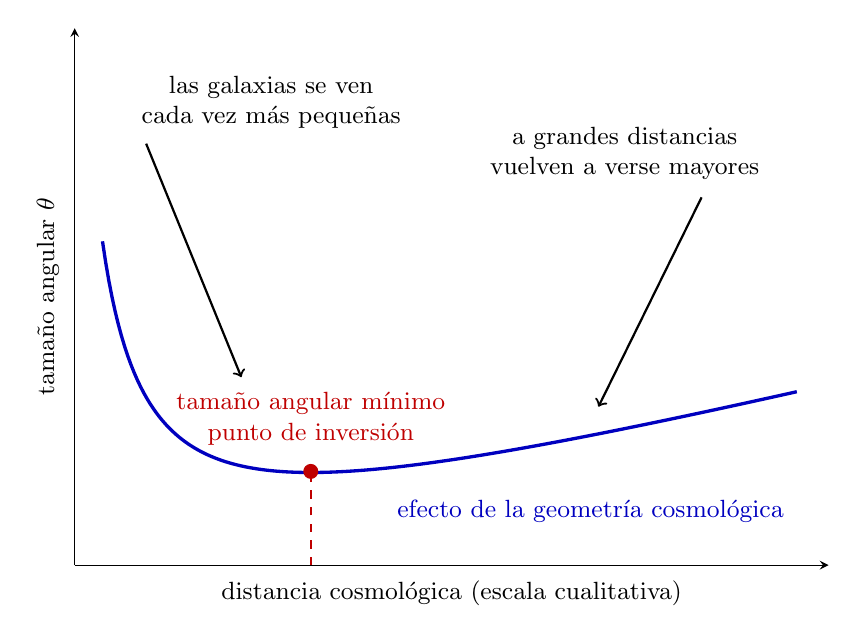
\begin{tikzpicture}
\begin{axis}[
    width=0.92\textwidth,
    height=8.4cm,
    xmin=0,
    xmax=9.5,
    ymin=0.35,
    ymax=2.35,
    axis lines=left,
    xlabel={distancia cosmológica (escala cualitativa)},
    ylabel={tamaño angular $\theta$},
    xtick=\empty,
    ytick=\empty,
    grid=major,
    grid style={gray!18},
    label style={font=\small},
    clip=false
]
    \addplot[blue!75!black,very thick,domain=0.35:9.1,samples=220]
        {0.78/(x+0.25)+0.075*x+0.23};

    \addplot[only marks,mark=*,mark size=2.5pt,red!75!black]
        coordinates {(2.975,0.699)};
    \draw[red!75!black,dashed,thick]
        (axis cs:2.975,0.35) -- (axis cs:2.975,0.699);
    \node[red!75!black,font=\small,align=center,anchor=south]
        at (axis cs:2.975,0.76)
        {tamaño angular mínimo\\punto de inversión};

    \draw[->,black,thick] (axis cs:0.9,1.92) -- (axis cs:2.1,1.05);
    \node[font=\small,align=center,anchor=south west]
        at (axis cs:0.72,1.94)
        {las galaxias se ven\\cada vez más pequeñas};

    \draw[->,black,thick] (axis cs:7.9,1.72) -- (axis cs:6.6,0.94);
    \node[font=\small,align=center,anchor=south east]
        at (axis cs:8.75,1.75)
        {a grandes distancias\\vuelven a verse mayores};

    \node[blue!75!black,font=\small]
        at (axis cs:6.5,0.55)
        {efecto de la geometría cosmológica};
\end{axis}
\end{tikzpicture}
\caption{Comportamiento cualitativo del tamaño angular de una galaxia de tamaño físico fijo al aumentar la distancia cosmológica. Inicialmente el tamaño angular disminuye, alcanza un mínimo y luego aumenta para objetos suficientemente lejanos, porque la relación entre distancia angular y corrimiento al rojo no es euclidiana en un universo en expansión.}
\label{fig:angular}
\end{figure}